\documentclass{acmsiggraph}                     % final
%Furthermore change the line \pagestyle{headings} to
%\pagestyle{empty}
\usepackage[scaled=.92]{helvet}

\usepackage{times}

\usepackage{graphicx}
\usepackage{amsmath}

%% The 'graphicx' package allows for the inclusion of EPS figures.

%% use this for zero \parindent and non-zero \parskip, intelligently.

\usepackage{parskip}

%% Optional: the 'caption' package provides a nicer-looking replacement
%% for the standard caption environment. With 'labelfont=bf,'textfont=it',
%% caption labels are bold and caption text is italic.

\usepackage[labelfont=bf,textfont=it]{caption}
\usepackage{subfig}

%% If you are submitting a paper to the annual conference, please replace
%% the value ``0'' below with the numeric value of your OnlineID.
%% If you are not submitting this paper to the annual conference,
%% you may safely leave it at ``0'' -- it will not be included in the output.

\onlineid{0}

%% Paper title.

\newcommand{\Eq}[1] {Eq.~(\ref{eq:#1})}
\newcommand{\Fig}[1]{Fig.~\ref{fig:#1}}
\newcommand{\Sec}[1]{Sec.~\ref{sec:#1}}
\newcommand{\Eqs}   {Eqs.~}
\newcommand{\Figs}  {Figs.~}
\newcommand{\Tbl}[1]{Table~\ref{tbl:#1}}
\newcommand{\Etal}  {{\it et al.}}
\newcommand{\Figa}[1]{Fig.~\ref{fig:#1}(a)}
\newcommand{\Figb}[1]{Fig.~\ref{fig:#1}(b)}
\newcommand{\Figc}[1]{Fig.~\ref{fig:#1}(c)}
\newcommand{\Figd}[1]{Fig.~\ref{fig:#1}(d)}

\graphicspath{{figures/}}

%%%%%% START OF THE PAPER %%%%%%

\begin{document}

\section{Model Comparison}
Although models generated by 3D BPA are of high resolution, they usually take a huge number of space
for storage. For example, the model depicted in \Fig{TH_BPA} needs almost 400 MB on space, which
prevents this solution from being applied to most of other applications, including web-based applications.
One way to improve the situation is to apply some approximation techniques to reduce the space required
by these models.
%%% Figure of the BPA snapshot
\begin{figure}[htbp]
\begin{center}
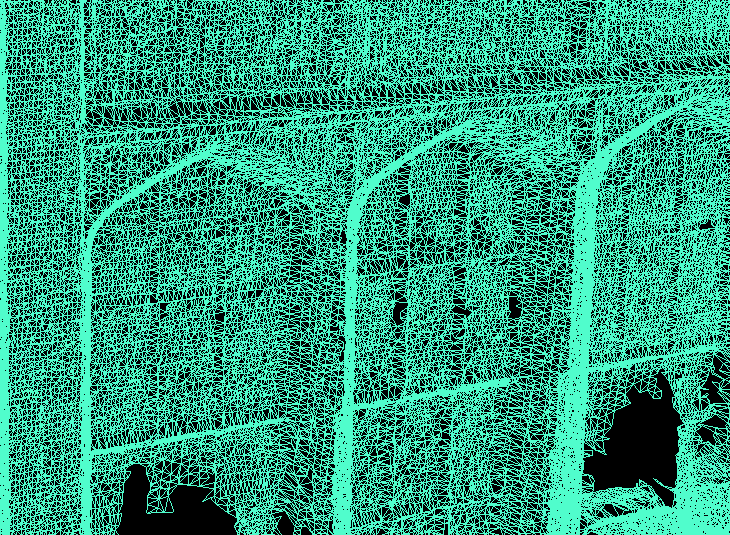
\includegraphics[width=3in]{BPA_TH.png}
\end{center}
\caption{The snapshot of the BPA model.}
\label{fig:TH_BPA}
\end{figure}
%%% End of Figure

Among all kinds of approximation approaches, {\it qslim} is one of the most sophisticated and efficient
approximation algorithm. So we carried out a comparison between models generated by our proposed
method and the models approximated by {\it qslim}. We compared these model under the same level of
approximation. In other words, the models under comparison are of approximate same number of model faces.
As a matter of fact, even for {\it qslim}, it ran out of memory on 3D model data generated by BPA of
the above example.
In order to reduce the size of the model for {\it qslim} to work, we have to either down-sampling the 3D model
generated by BPA or split it into sub-models which can be handled by {\it qslim}.

%%% Figure of the comparison
\begin{figure}[htbp]
\begin{center}
\begin{tabular}{cc}
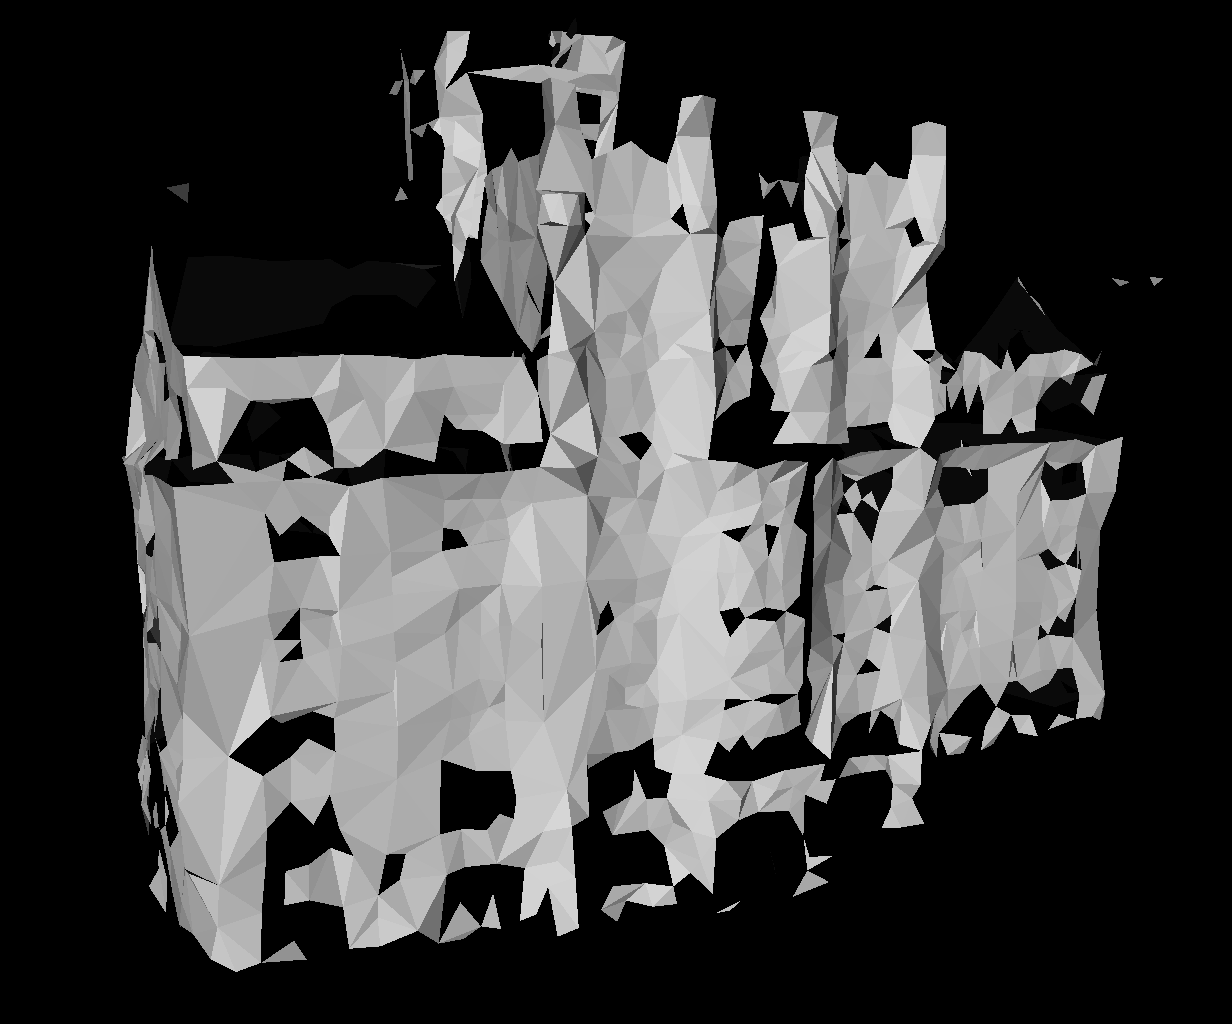
\includegraphics[width=0.2\textwidth]{comp_32_2_qslim.png} &
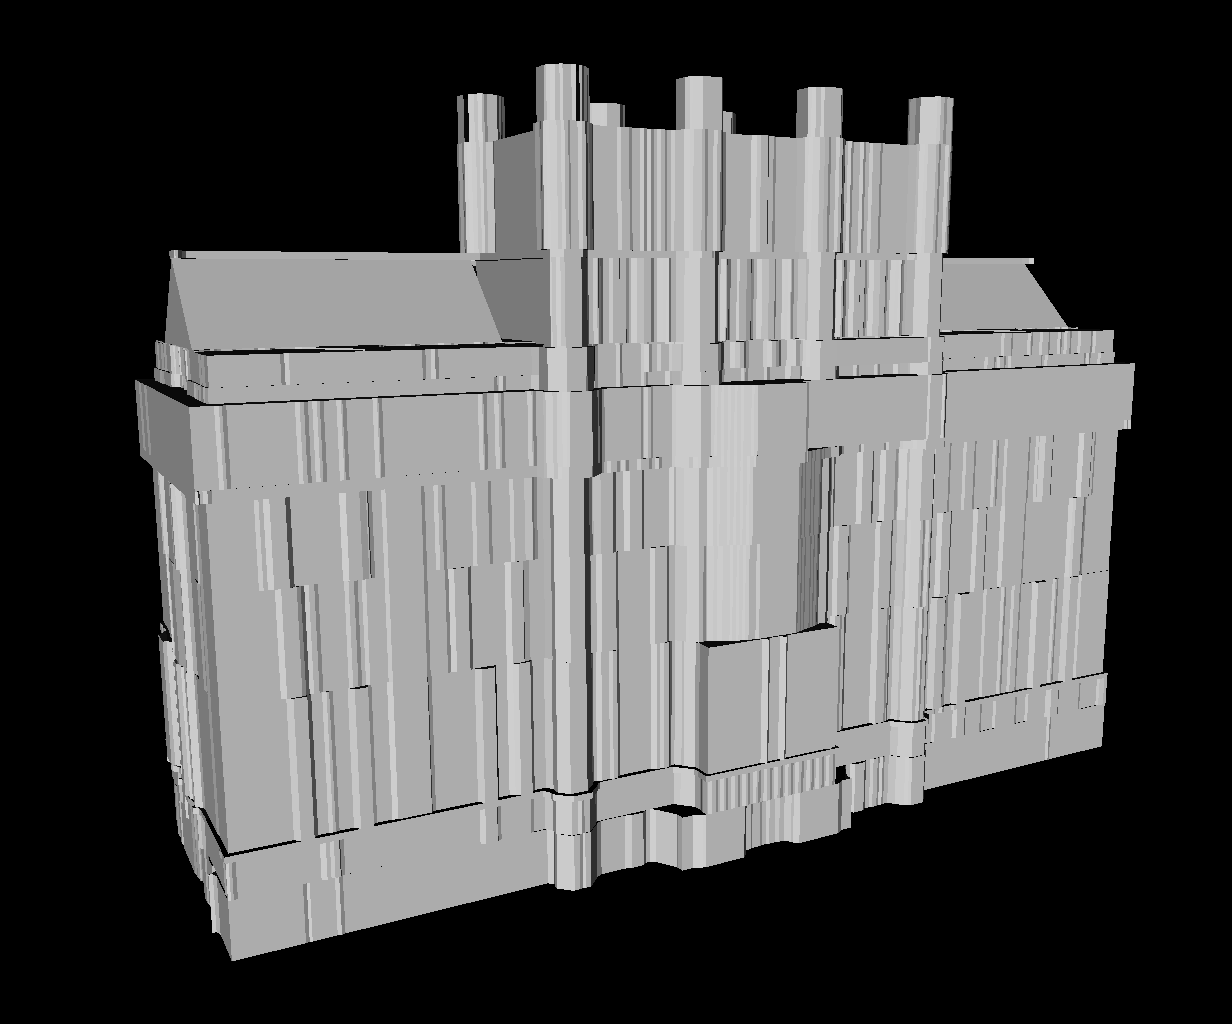
\includegraphics[width=0.2\textwidth]{comp_32_2.png} \\
(a) & (b) \\
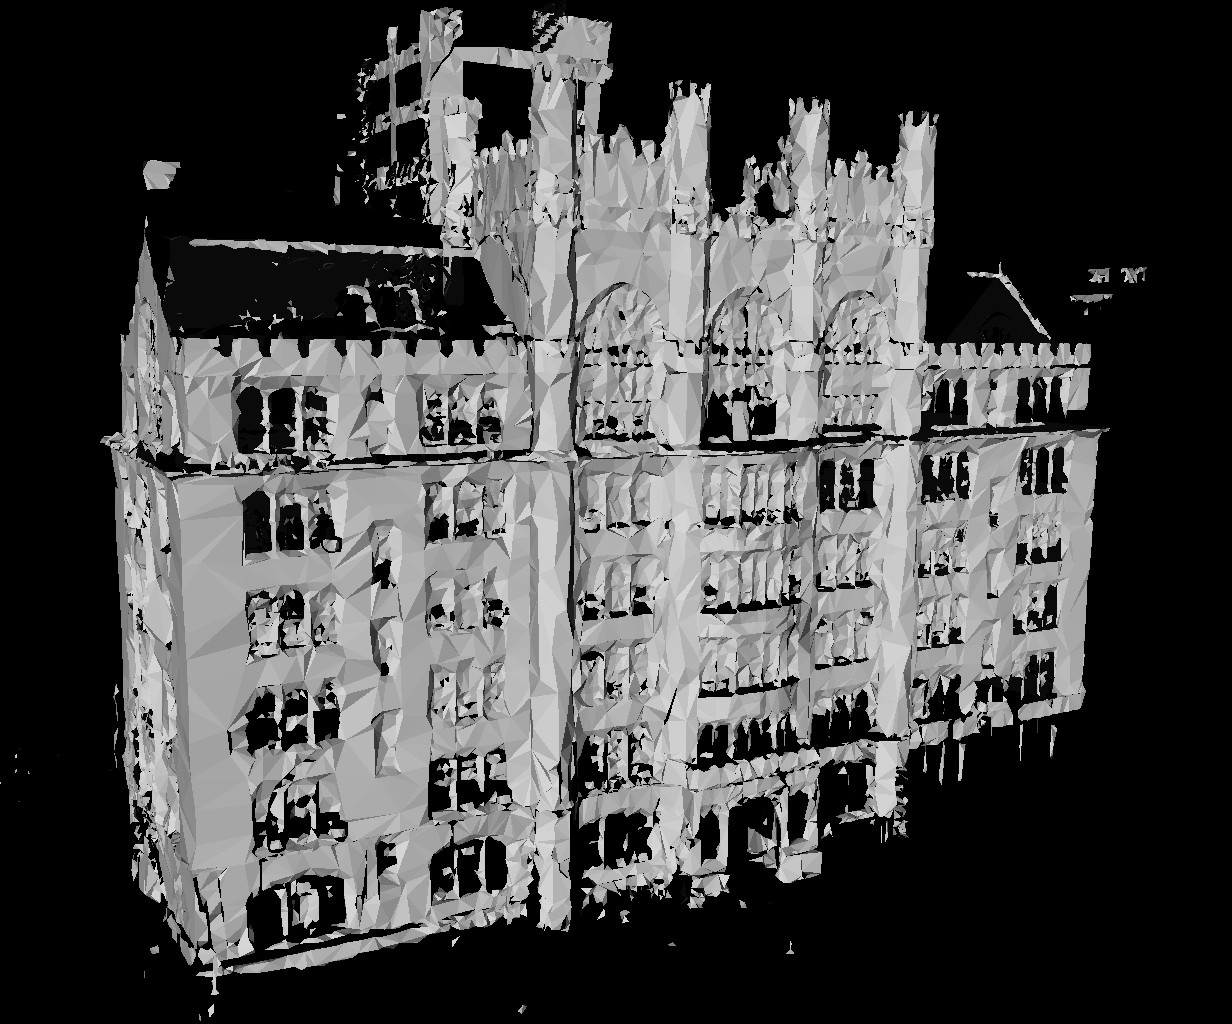
\includegraphics[width=0.2\textwidth]{comp_4_2_qslim.png} &
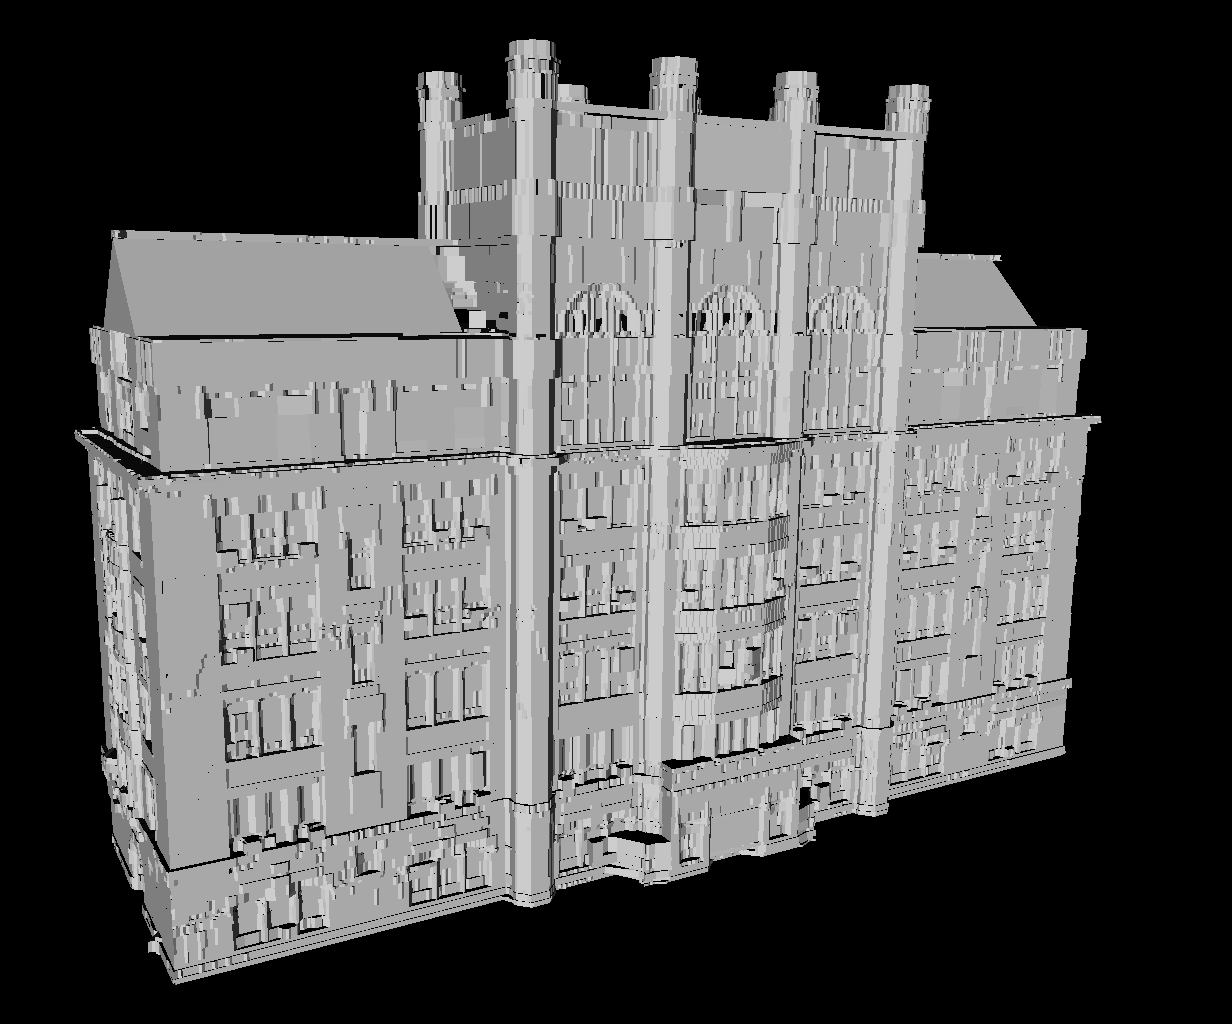
\includegraphics[width=0.2\textwidth]{comp_4_2.png} \\
(c) & (d)
\end{tabular}
\end{center}
\caption{The models with 2,000 faces generated by (a) {\it qslim} (b) our proposed approach. as well as with 32,000 faces
generated by (c) {\it qslim} and (d) our proposed approach.}
\label{fig:TH_comp}
\end{figure}
%%% End of Figure

\Figa{TH_comp} and \Figb{TH_comp} shows the snapshots of models generated by {\it qslim} and our proposed
method with approximate 2,000 faces. A relative high resolution models with roughly 32,000
faces are shown in \Figc{TH_comp} and \Figd{TH_comp}. As we can see the models approximated by {\it qslim}
are not as good as ours in a sense that their models are not able to preserve the sharpness of the
original model.



\end{document}
